\chapter{Testy}

\section{Testy integracyjne}

Testy integracyjne mają na celu sprawdzenie, czy interfejsy pomiędzy komponentami współdziałają ze sobą poprawnie.\cite{mielnikIntegrationTests} Do przeprowadzenia testów została użyta biblioteka "pytest", która pozwala na szybkie i proste uruchomienie testów.\cite{oliveira2018} Do wykonywania zapytań HTTP została wykorzystana biblioteka "requests". Testy miały na celu sprawdzenie, czy status zwrócony przez wykonane żądanie pokrywa się z oczekiwanym rezultatem.\\
Przetestowane zostały poniższe funkcjonalności systemu:

\begin{itemize}
    \item Utworzenie fiszki
    \item Zwrócenie danych fiszki na podstawie id
    \item Aktualizacja danych fiszki
    \item Usunięcie fiszki
    \item Otrzymanie odpowiedzi od chatu GPT
    \item Tworzenie talii
    \item Zwrócenie danych talii na podstawie id
    \item Zwrócenie danych wszystkich talii należących do użytkownika
    \item Aktualizacja danych talii
    \item Usunięcie talii
    \item Zwrócenie rankingu talii
    \item Utworzenie konta użytkownika
    \item Logowanie do systemu
    \item Zwrócenie danych użytkownika
\end{itemize}

\begin{figure}[H]
    \centering
    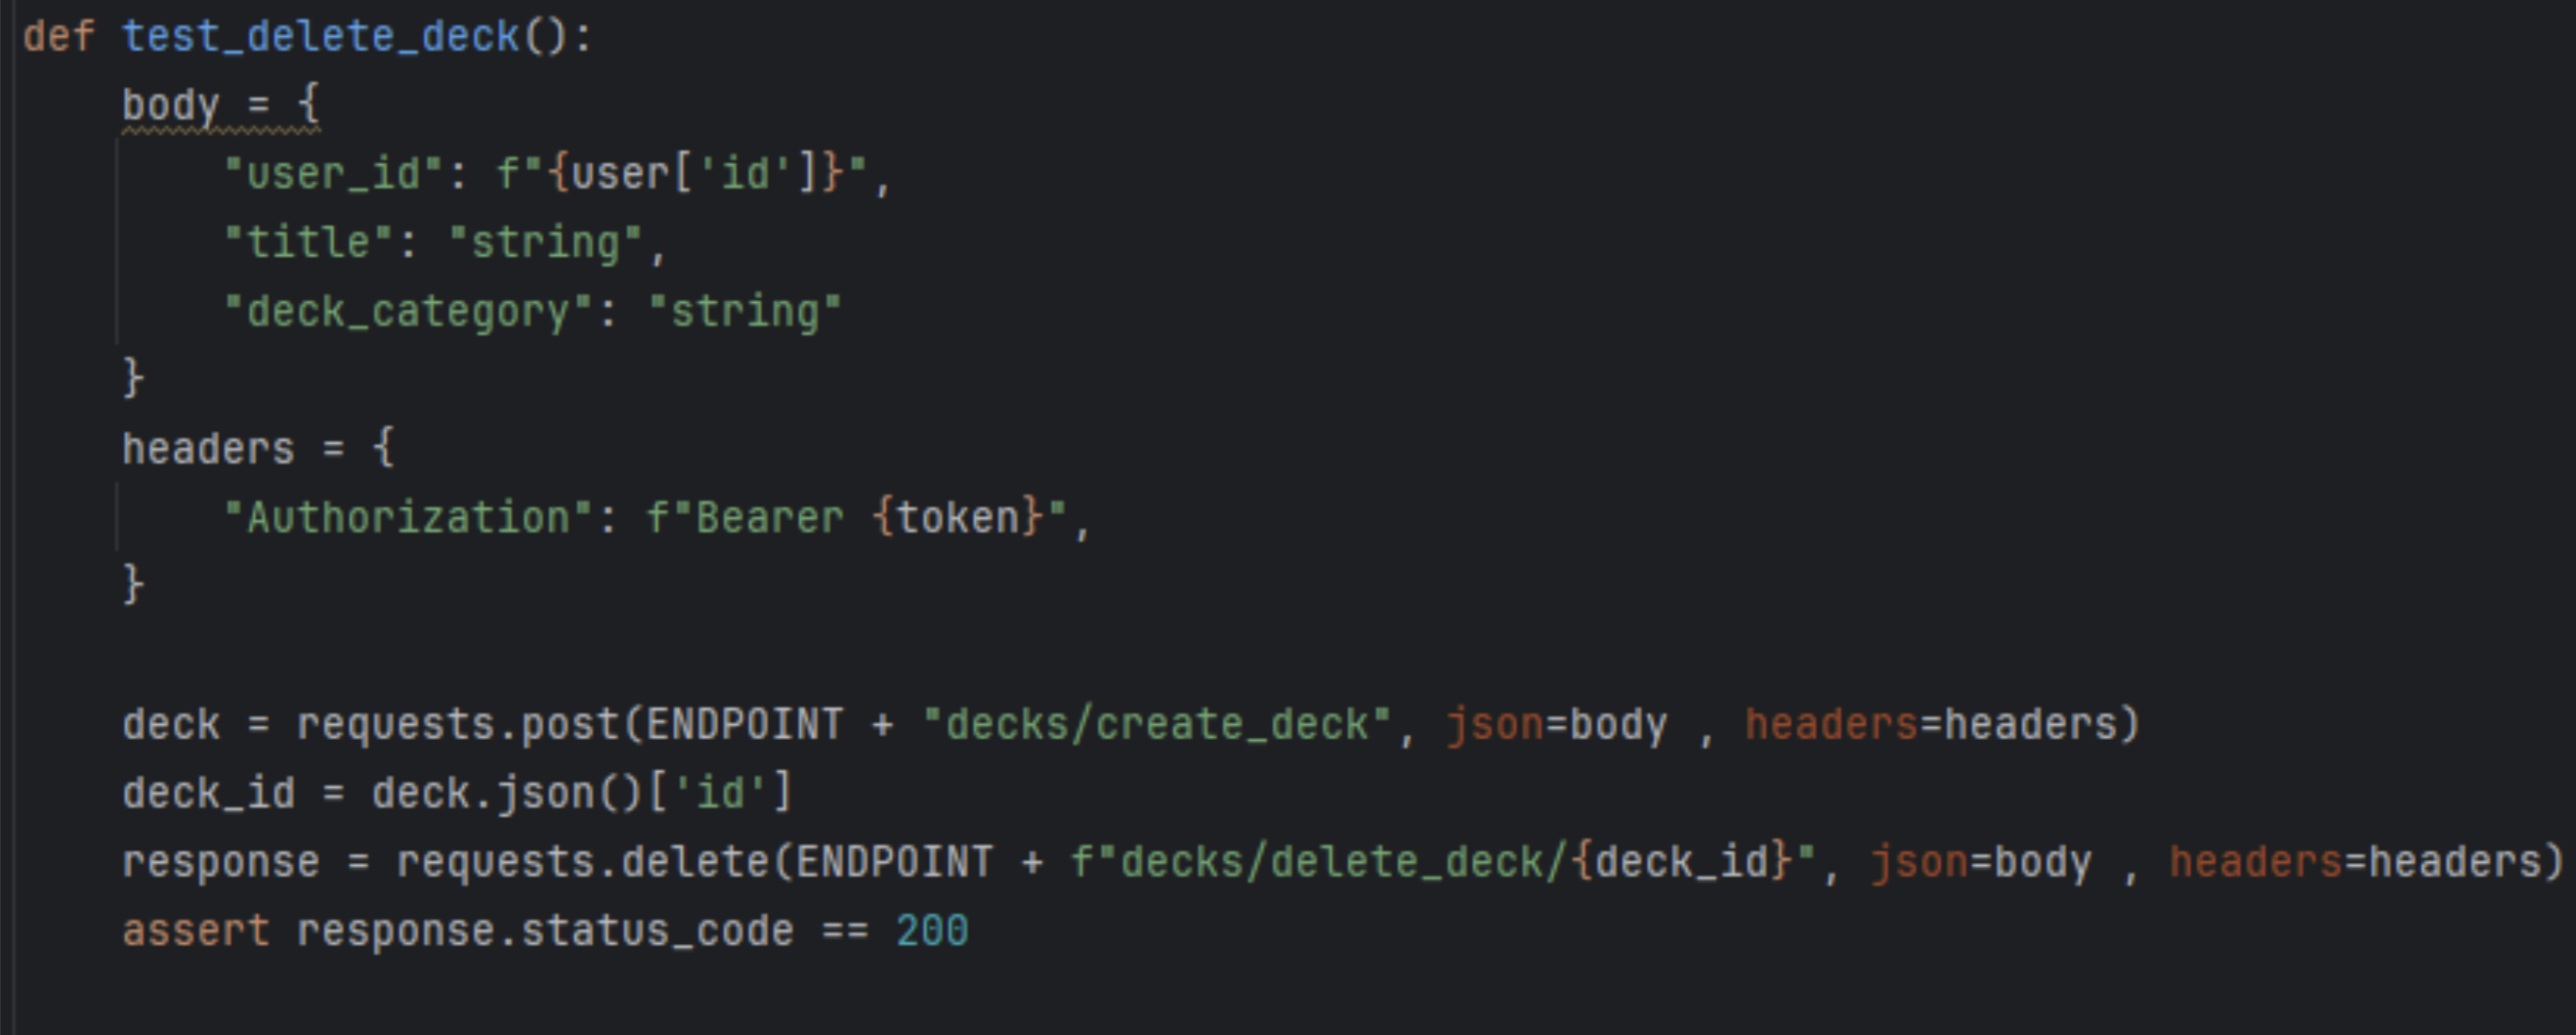
\includegraphics[width=1\textwidth]{chapters/chapter_9/testy1}
    \caption{Test sprawdzający działanie endpointu do usuwania talii użytkownika.}
    \label{img:testy}
\end{figure}

\section{Testy akceptacyjne}

Testy akceptacyjne pozwalają ocenić gotowość systemu do wdrożenia. Głównym ich założeniem jest sprawdzenie, czy system nadaje się do użytkowania.\cite{acceptanceTesting} Do przeprowadzenia testów zostały sporządzone scenariusze testowe. Oliwier przechodził przez scenariusze testowe w celu sprawdzenia czy aplikacja działa zgodnie z oczekiwaniami.


\begin{table}[H]
\centering
\begin{tabularx}{\textwidth}{|>{\raggedright\arraybackslash}p{0.3\textwidth}|X|}
    \hline
    \textbf{Opis przypadku:} & Rejestracja użytkownika na stronie internetowej \\
    \hline
    \textbf{Cel przypadku:} & Użytkownik rejestruje się aby utworzyć konto, potrzebne do logowania. \\
    \hline
    \textbf{Testowane wymagania:} & 3.2.1 Tworzenie konta użytkownika \\
    \hline
    \textbf{Warunki początkowe:} & Strona z formularzem, która pozwala wprowadzić dane użytkownika w celu zarejestrowania go. \\
    \hline
    \textbf{Warunki końcowe:} & Utworzone konto użytkownika \\
    \hline
    \textbf{Dane wejściowe:} & E-mail użytkownika, hasło i nickname \\
    \hline
    \textbf{Oczekiwany wynik:} & Użytkownik po zarejestrowaniu zostanie dodany do bazy danych a utworzone konto pozwoli mu na logowanie do strony. \\
    \hline
    \textbf{Kroki procedury:} &
        1. Uruchomienie przeglądarki - \textbf{Pozytywny} \newline
        2. Wejście na stronę rejestracji - \textbf{Pozytywny} \newline
        3. Wypełnienie formularza rejestracji - \textbf{Pozytywny} \newline
        4. Kliknięcie w przycisk rejestracji - \textbf{Pozytywny} \newline
        5. Nowe konto dodane do bazy danych - \textbf{Pozytywny} \\
    \hline
    \textbf{Wynik:} & \textbf{Pozytywny} \\
    \hline
\end{tabularx}
    \caption{Test akceptacyjny procesu rejestracji nowego użytkownika.}
\end{table}


\begin{table}[ht]
\centering
\begin{tabularx}{\textwidth}{|>{\raggedright\arraybackslash}p{0.3\textwidth}|X|}
    \hline
    \textbf{Opis przypadku:} & Logowanie na stronę \\
    \hline
    \textbf{Cel przypadku:} & Sprawdzenie czy użytkownik posiadający konto ma dostęp do strony po poprawnym wypełnieniu formularza logowania. \\
    \hline
    \textbf{Testowane wymagania:} & 3.2.2 Logowanie do systemu \\
    \hline
    \textbf{Warunki początkowe:} & Posiadane konto użytkownika \\
    \hline
    \textbf{Warunki końcowe:} & dostęp do strony domowej \\
    \hline
    \textbf{Dane wejściowe:} & email, hasło \\
    \hline
    \textbf{Oczekiwany wynik:} & Użytkownik po poprawnym zalogowaniu przechodzi do strony domowej. \\
    \hline
    \textbf{Kroki procedury:} &
        1. Uruchomienie przeglądarki - \textbf{Pozytywny} \newline
        2. Wejście na stronę logowania - \textbf{Pozytywny} \newline
        3. Wypełnienie formularza logowania - \textbf{Pozytywny} \newline
        4. Użytkownik zostaje przekierowany do strony domowej - \textbf{Pozytywny} \\
    \hline
    \textbf{Wynik:} & \textbf{Pozytywny} \\
    \hline
\end{tabularx}
    \caption{Test akceptacyjny procesu logowania użytkownika.}
\end{table}


\begin{table}[ht]
\centering
\begin{tabularx}{\textwidth}{|>{\raggedright\arraybackslash}p{0.3\textwidth}|X|}
    \hline
    \textbf{Opis przypadku:} & Wylogowanie z systemu \\
    \hline
    \textbf{Cel przypadku:} & Sprawdzenie czy po wylogowaniu użytkownik, nie ma dostęp do strony domowej bez ponownego zalogowania \\
    \hline
    \textbf{Testowane wymagania:} & 3.2.3 Wylogowanie z systemu \\
    \hline
    \textbf{Warunki początkowe:} & Posiadane konto użytkownika \\
    \hline
    \textbf{Warunki końcowe:} & Użytkownik po kliknięciu przycisku wylogowania zostaje przekierowany do strony logowania i nie ma dostęp do strony domowej bez ponownego zalogowania \\
    \hline
    \textbf{Dane wejściowe:} & email, hasło \\
    \hline
    \textbf{Oczekiwany wynik:} & Brak dostępu do strony domowej \\
    \hline
    \textbf{Kroki procedury:} &
        1. Uruchomienie przeglądarki - \textbf{Pozytywny} \newline
        2. Wejście na stronę logowania - \textbf{Pozytywny} \newline
        3. Wypełnienie formularza logowania - \textbf{Pozytywny} \newline
        4. Użytkownik zostaje przekierowany do strony domowej - \textbf{Pozytywny} \newline
        5. Kliknięcie w logout na nawigacji - \textbf{Pozytywny} \newline
        6. Przekierowanie do strony logowania - \textbf{Pozytywny} \\
    \hline
    \textbf{Wynik:} & \textbf{Pozytywny} \\
    \hline
\end{tabularx}
    \caption{Test akceptacyjny procesu wylogowania użytkownika.}
\end{table}


\begin{table}[ht]
\centering
\begin{tabularx}{\textwidth}{|>{\raggedright\arraybackslash}p{0.3\textwidth}|X|}
    \hline
    \textbf{Opis przypadku:} & Edycja adresu email \\
    \hline
    \textbf{Cel przypadku:} & Sprawdzenie czy użytkownik może zmienić email \\
    \hline
    \textbf{Testowane wymagania:} & 3.2.4 Edycja danych użytkownika \\
    \hline
    \textbf{Warunki początkowe:} & Posiadane konto użytkownika \\
    \hline
    \textbf{Warunki końcowe:} & Dane użytkownika zostaną zaktualizowane \\
    \hline
    \textbf{Dane wejściowe:} & email, hasło \\
    \hline
    \textbf{Oczekiwany wynik:} & Użytkownik po zmianie email zostaje wylogowany, a email zostanie zaktualizowany. \\
    \hline
    \textbf{Kroki procedury:} &
        1. Uruchomienie przeglądarki - \textbf{Pozytywny} \newline
        2. Wejście na stronę logowania - \textbf{Pozytywny} \newline
        3. Wypełnienie formularza logowania - \textbf{Pozytywny} \newline
        4. Użytkownik zostaje przekierowany do strony domowej - \textbf{Pozytywny} \newline
        5. Kliknięcie w profil użytkownika - \textbf{Pozytywny} \newline
        6. Kliknięcie w przycisk zmiany email - \textbf{Pozytywny} \newline
        7. Wypełnienie formularza i kliknięcie zapisu - \textbf{Pozytywny} \newline
        8. Przekierowanie do strony logowania - \textbf{Pozytywny} \newline
        9. Zalogowanie się przy użyciu nowych danych - \textbf{Pozytywny} \\
    \hline
    \textbf{Wynik:} & \textbf{Pozytywny} \\
    \hline
\end{tabularx}
    \caption{Test zmiany adresu email użytkownika.}
\end{table}


\begin{table}[ht]
\centering
\begin{tabularx}{\textwidth}{|>{\raggedright\arraybackslash}p{0.3\textwidth}|X|}
    \hline
    \textbf{Opis przypadku:} & Usunięcie konta użytkownika \\
    \hline
    \textbf{Cel przypadku:} & Sprawdzenie czy użytkownik może usunąć swoje konto. \\
    \hline
    \textbf{Testowane wymagania:} & 3.2.5 Usunięcie konta użytkownika \\
    \hline
    \textbf{Warunki początkowe:} & Posiadane konto użytkownika \\
    \hline
    \textbf{Warunki końcowe:} & usunięte konto użytkownika, brak możliwości zalogowania \\
    \hline
    \textbf{Dane wejściowe:} & email, hasło \\
    \hline
    \textbf{Oczekiwany wynik:} & Użytkownik po usunięciu konta zostaje wylogowany z aplikacji. \\
    \hline
    \textbf{Kroki procedury:} &
        1. Uruchomienie przeglądarki - \textbf{Pozytywny} \newline
        2. Wejście na stronę logowania - \textbf{Pozytywny} \newline
        3. Wypełnienie formularza logowania - \textbf{Pozytywny} \newline
        4. Użytkownik zostaje przekierowany do strony domowej - \textbf{Pozytywny} \newline
        5. Kliknięcie w profil użytkownika - \textbf{Pozytywny} \newline
        6. Kliknięcie w usunięcie konta - \textbf{Pozytywny} \newline
        7. Wypełnienie formularza i kliknięcie zapisu - \textbf{Pozytywny} \newline
        8. Przekierowanie do strony logowania - \textbf{Pozytywny} \newline
        9. Użytkownik nie jest w stanie zalogować się do strony - \textbf{Pozytywny} \\
    \hline
    \textbf{Wynik:} & \textbf{Pozytywny} \\
    \hline
\end{tabularx}
    \caption{Test procesu usuwania konta użytkownika.}
\end{table}


\begin{table}[ht]
\centering
\begin{tabularx}{\textwidth}{|>{\raggedright\arraybackslash}p{0.3\textwidth}|X|}
    \hline
    \textbf{Opis przypadku:} & Tworzenie talii fiszek \\
    \hline
    \textbf{Cel przypadku:} & Sprawdzenie czy użytkownik może utworzyć nową talię fiszek. \\
    \hline
    \textbf{Testowane wymagania:} & 3.2.6 Tworzenie talii fiszek \\
    \hline
    \textbf{Warunki początkowe:} & Posiadane konto użytkownika \\
    \hline
    \textbf{Warunki końcowe:} & Utworzona talia fiszek \\
    \hline
    \textbf{Dane wejściowe:} & nazwa i kategoria talii, treść fiszki \\
    \hline
    \textbf{Oczekiwany wynik:} & Po utworzeniu talii jest ona dostępna na podstronie my decks. \\
    \hline
    \textbf{Kroki procedury:} &
        1. Uruchomienie przeglądarki - \textbf{Pozytywny} \newline
        2. Wejście na stronę logowania - \textbf{Pozytywny} \newline
        3. Wypełnienie formularza logowania - \textbf{Pozytywny} \newline
        4. Użytkownik zostaje przekierowany do strony domowej - \textbf{Pozytywny} \newline
        5. Kliknięcie w create decks - \textbf{Pozytywny} \newline
        6. Użytkownik wypełnia pole z nazwą i kategorią talii - \textbf{Pozytywny} \newline
        7. Wypełnienie przedniej i tylnej strony fiszki - \textbf{Pozytywny} \newline
        8. Kliknięcie w przycisk create deck - \textbf{Pozytywny} \newline
        9. Przejście do strony domowej - \textbf{Pozytywny} \newline
        10. Przejście do strony my decks w celu sprawdzenia czy została dodana utworzona talia - \textbf{Pozytywny} \\
    \hline
    \textbf{Wynik:} & \textbf{Pozytywny} \\
    \hline
\end{tabularx}
    \caption{Test procesu tworzenia nowej talii fiszek.}
\end{table}


\begin{table}[ht]
\centering
\begin{tabularx}{\textwidth}{|>{\raggedright\arraybackslash}p{0.3\textwidth}|X|}
    \hline
    \textbf{Opis przypadku:} & Usunięcie talii fiszek \\
    \hline
    \textbf{Cel przypadku:} & Sprawdzenie czy użytkownik, może usunąć talie, która nie jest mu już potrzebna \\
    \hline
    \textbf{Testowane wymagania:} & 3.2.7 Usunięcie talii fiszek \\
    \hline
    \textbf{Warunki początkowe:} & Posiadane konto użytkownika, utworzona talia \\
    \hline
    \textbf{Warunki końcowe:} & Talia przestaje istnieć \\
    \hline
    \textbf{Dane wejściowe:} & Brak \\
    \hline
    \textbf{Oczekiwany wynik:} & Po usunięciu talia znika z podstrony my decks \\
    \hline
    \textbf{Kroki procedury:} &
        1. Uruchomienie przeglądarki - \textbf{Pozytywny} \newline
        2. Wejście na stronę logowania - \textbf{Pozytywny} \newline
        3. Wypełnienie formularza logowania - \textbf{Pozytywny} \newline
        4. Użytkownik zostaje przekierowany do strony domowej - \textbf{Pozytywny} \newline
        5. Kliknięcie w my decks - \textbf{Pozytywny} \newline
        6. Kliknięcie w talie - \textbf{Pozytywny} \newline
        7. Kliknięcie w opcję - \textbf{Pozytywny} \newline
        8. Kliknięcie w delete deck i potwierdzenie usunięcia decku - \textbf{Pozytywny} \newline
        9. Przekierowanie do strony my decks. Brak widocznej talii na stronie my decks - \textbf{Pozytywny} \\
    \hline
    \textbf{Wynik:} & \textbf{Pozytywny} \\
    \hline
\end{tabularx}
    \caption{Test procesu usuwania talii fiszek.}
\end{table}


\begin{table}[ht]
\centering
\begin{tabularx}{\textwidth}{|>{\raggedright\arraybackslash}p{0.3\textwidth}|X|}
    \hline
    \textbf{Opis przypadku:} & Edycja talii fiszek \\
    \hline
    \textbf{Cel przypadku:} & Użytkownik musi mieć możliwość zmiany nazwy talii lub kategorii, jeżeli popełni jakiś błąd w tytule lub kategorii. \\
    \hline
    \textbf{Testowane wymagania:} & 3.2.8 Edycja talii fiszek \\
    \hline
    \textbf{Warunki początkowe:} & Utworzona talia fiszek \\
    \hline
    \textbf{Warunki końcowe:} & Talia fiszek zaktualizowana o nowe wartości. \\
    \hline
    \textbf{Dane wejściowe:} & Brak \\
    \hline
    \textbf{Oczekiwany wynik:} & Zostaje zmieniona nazwa talii i kategoria. \\
    \hline
    \textbf{Kroki procedury:} &
        1. Uruchomienie przeglądarki - \textbf{Pozytywny} \newline
        2. Wejście na stronę logowania - \textbf{Pozytywny} \newline
        3. Wypełnienie formularza logowania - \textbf{Pozytywny} \newline
        4. Użytkownik zostaje przekierowany do strony domowej - \textbf{Pozytywny} \newline
        5. Kliknięcie w my decks - \textbf{Pozytywny} \newline
        6. Kliknięcie w talie - \textbf{Pozytywny} \newline
        7. Kliknięcie w opcje - \textbf{Pozytywny} \newline
        8. Kliknięcie w zmianę kategorii lub nazwy - \textbf{Pozytywny} \newline
        9. Podanie w formularzu nowych wartości dla kategorii i nazwy - \textbf{Pozytywny} \newline
        10. Kliknięcie w przycisk save - \textbf{Pozytywny} \newline
        11. Informacje talii zostaną zaktualizowane o nowe wartości - \textbf{Pozytywny} \\
    \hline
    \textbf{Wynik:} & \textbf{Pozytywny} \\
    \hline
\end{tabularx}
    \caption{Test procesu edycji talii fiszek.}
\end{table}


\begin{table}[ht]
\centering
\begin{tabularx}{\textwidth}{|>{\raggedright\arraybackslash}p{0.3\textwidth}|X|}
    \hline
    \textbf{Opis przypadku:} & Tryb uczenia się z talii fiszek służy do podziału fiszek na te, które użytkownik zna i te nie zapamiętane \\
    \hline
    \textbf{Cel przypadku:} & Sprawdzenie czy tryb uczenia poprawnie rozdziela fiszki należące do talii \\
    \hline
    \textbf{Testowane wymagania:} & 3.2.9 Tryb uczenia się z talii fiszek \\
    \hline
    \textbf{Warunki początkowe:} & Utworzona talia fiszek, posiadane konto użytkownika \\
    \hline
    \textbf{Warunki końcowe:} & Fiszki podzielone na zapamiętane i nie zapamiętane \\
    \hline
    \textbf{Dane wejściowe:} & Brak \\
    \hline
    \textbf{Oczekiwany wynik:} & Fiszki w talii zostają podzielone przez użytkownika na te, które zna i te których nie pamięta \\
    \hline
    \textbf{Kroki procedury:} &
        1. Uruchomienie przeglądarki - \textbf{Pozytywny} \newline
        2. Wejście na stronę logowania - \textbf{Pozytywny} \newline
        3. Wypełnienie formularza logowania - \textbf{Pozytywny} \newline
        4. Użytkownik zostaje przekierowany do strony domowej - \textbf{Pozytywny} \newline
        5. Kliknięcie w my decks - \textbf{Pozytywny} \newline
        6. Kliknięcie w talie - \textbf{Pozytywny} \newline
        7. Kliknięcie w tryb uczenia się - \textbf{Pozytywny} \newline
        8. Użytkownik dzieli talię na fiszki, na zapamiętane i nie zapamiętane - \textbf{Pozytywny} \newline
        9. Fiszki w talii zostają podzielone na zapamiętane i nie zapamiętane - \textbf{Pozytywny} \\
    \hline
    \textbf{Wynik:} & \textbf{Pozytywny} \\
    \hline
\end{tabularx}
    \caption{Test trybu uczenia się z talii fiszek.}
\end{table}


\begin{table}[ht]
\centering
\begin{tabularx}{\textwidth}{|>{\raggedright\arraybackslash}p{0.3\textwidth}|X|}
    \hline
    \textbf{Opis przypadku:} & Po uruchomieniu trybu sterowania głosowego, aplikacja powinna reagować na komendy głosowe \\
    \hline
    \textbf{Cel przypadku:} & Sprawdzenie czy aplikacja reaguje na komendy głosowe \\
    \hline
    \textbf{Testowane wymagania:} & 3.2.10 Sterowanie talią przy użyciu mowy \\
    \hline
    \textbf{Warunki początkowe:} & Utworzona talia fiszek, posiadane konto użytkownika \\
    \hline
    \textbf{Warunki końcowe:} & Brak \\
    \hline
    \textbf{Dane wejściowe:} & Brak \\
    \hline
    \textbf{Oczekiwany wynik:} & Aplikacja wykonuje akcje zgodnie z wypowiedzianymi przez użytkownika komendami \\
    \hline
    \textbf{Kroki procedury:} &
        1. Uruchomienie przeglądarki - \textbf{Pozytywny} \newline
        2. Wejście na stronę logowania - \textbf{Pozytywny} \newline
        3. Wypełnienie formularza logowania - \textbf{Pozytywny} \newline
        4. Użytkownik zostaje przekierowany do strony domowej - \textbf{Pozytywny} \newline
        5. Kliknięcie w my decks - \textbf{Pozytywny} \newline
        6. Kliknięcie w talie - \textbf{Pozytywny} \newline
        7. Kliknięcie w voice control - \textbf{Pozytywny} \newline
        8. Kliknięcie w start listening - \textbf{Pozytywny} \newline
        9. Pojawia się popup box z instrukcją, zamknięcie instrukcji powoduje rozpoczęcie nasłuchiwania przez mikrofon - \textbf{Pozytywny} \newline
        10. Komenda "next flashcard" przenosi do następnej fiszki - \textbf{Pozytywny} \newline
        11. Komenda "read text" uruchamia syntezator odczytujący treść fiszki - \textbf{Pozytywny} \newline
        12. Komenda "rotate" obraca fiszkę - \textbf{Pozytywny} \newline
        13. Komenda "previous flashcard" przenosi do poprzedniej fiszki - \textbf{Pozytywny} \newline
        14. Komenda "stop control" wyłącza tryb głosowy - \textbf{Pozytywny} \\
    \hline
    \textbf{Wynik:} & \textbf{Pozytywny} \\
    \hline
\end{tabularx}
    \caption{Test sterowania talią przy użyciu mowy.}
\end{table}


\begin{table}[ht]
\centering
\begin{tabularx}{\textwidth}{|>{\raggedright\arraybackslash}p{0.3\textwidth}|X|}
    \hline
    \textbf{Opis przypadku:} & Import talii pozwala na dodanie talii znalezionej w rankingu do talii zawartych w public decks \\
    \hline
    \textbf{Cel przypadku:} & Sprawdzenie czy talia zaimportowana z rankingu dodaje się do public decks \\
    \hline
    \textbf{Testowane wymagania:} & 3.2.11 Import talii innych użytkowników \\
    \hline
    \textbf{Warunki początkowe:} & Utworzone konto użytkownika \\
    \hline
    \textbf{Warunki końcowe:} & Talia dodana do public decks \\
    \hline
    \textbf{Dane wejściowe:} & Brak \\
    \hline
    \textbf{Oczekiwany wynik:} & Po kliknięciu przycisku importuj talia fiszek zostaje dodana do public decks \\
    \hline
    \textbf{Kroki procedury:} &
        1. Uruchomienie przeglądarki - \textbf{Pozytywny} \newline
        2. Wejście na stronę logowania - \textbf{Pozytywny} \newline
        3. Wypełnienie formularza logowania - \textbf{Pozytywny} \newline
        4. Użytkownik zostaje przekierowany do strony domowej - \textbf{Pozytywny} \newline
        5. Kliknięcie w ranking na nawigacji - \textbf{Pozytywny} \newline
        6. Kliknięcie w decks ranking - \textbf{Pozytywny} \newline
        7. Kliknięcie w dowolną talię - \textbf{Pozytywny} \newline
        8. Kliknięcie w przycisk import deck - \textbf{Pozytywny} \newline
        9. Przeniesienie użytkownika do public decks - \textbf{Pozytywny} \newline
        10. Zaimportowana talia dodana do public decks - \textbf{Pozytywny} \\
    \hline
    \textbf{Wynik:} & \textbf{Pozytywny} \\
    \hline
\end{tabularx}
    \caption{Test procesu importowania talii fiszek z rankingu.}
\end{table}


\begin{table}[ht]
\centering
\begin{tabularx}{\textwidth}{|>{\raggedright\arraybackslash}p{0.3\textwidth}|X|}
    \hline
    \textbf{Opis przypadku:} & Użytkownik może wykorzystać przycisk generowania treści w celu wygenerowania przez chat GPT zawartości fiszki. \\
    \hline
    \textbf{Cel przypadku:} & Sprawdzenie czy treść fiszki zostaje wygenerowana. \\
    \hline
    \textbf{Testowane wymagania:} & 3.2.16 Generowanie treści fiszki na podstawie słów kluczowych \\
    \hline
    \textbf{Warunki początkowe:} & Utworzone kont użytkownika \\
    \hline
    \textbf{Warunki końcowe:} & Wygenerowana treść fiszki \\
    \hline
    \textbf{Dane wejściowe:} & Wpisanie treści w przednią część fiszki \\
    \hline
    \textbf{Oczekiwany wynik:} & Po uzupełnieniu przedniej strony fiszki i kliknięciu generate zostanie wyświetlona treść wygenerowana przez chat GPT. \\
    \hline
    \textbf{Kroki procedury:} &
        1. Uruchomienie przeglądarki - \textbf{Pozytywny} \newline
        2. Wejście na stronę logowania - \textbf{Pozytywny} \newline
        3. Wypełnienie formularza logowania - \textbf{Pozytywny} \newline
        4. Użytkownik zostaje przekierowany do strony domowej - \textbf{Pozytywny} \newline
        5. Kliknięcie w create decks - \textbf{Pozytywny} \newline
        6. Uzupełnienie przedniej strony fiszki treścią - \textbf{Pozytywny} \newline
        7. Kliknięcie w generate - \textbf{Pozytywny} \newline
        8. Pojawienie się okienka z wygenerowaną treścią - \textbf{Pozytywny} \newline
        9. Kliknięcie accept - \textbf{Pozytywny} \newline
        10. Tylna część fiszki zostaje uzupełniona wygenerowaną treścią - \textbf{Pozytywny} \\
    \hline
    \textbf{Wynik:} & \textbf{Pozytywny} \\
    \hline
\end{tabularx}
    \caption{Test generowania treści fiszki przy użyciu funkcji ChatGPT.}
\end{table}


